\section{Pre-processing}

\begin{itemize}
\item The data set can be found in an arff format at \\ \href{github.com/ongxuanhong/Preprocessing-with-horse-colic-dataset/blob/master/horse-colic.arff}{https://github.com/ongxuanhong/Preprocessing-with-horse-colic-dataset/blob/master/horse-colic.arff}
\end{itemize}
The data set we have chosen belongs to the field of veterinary medicine. More specifically, horse health. Successful association rule analysis has the potential to help veterinarians with diagnosis and  to evaluate treatment.\\
Below is a visualization of the data.
\begin{figure}[h!]
\centering
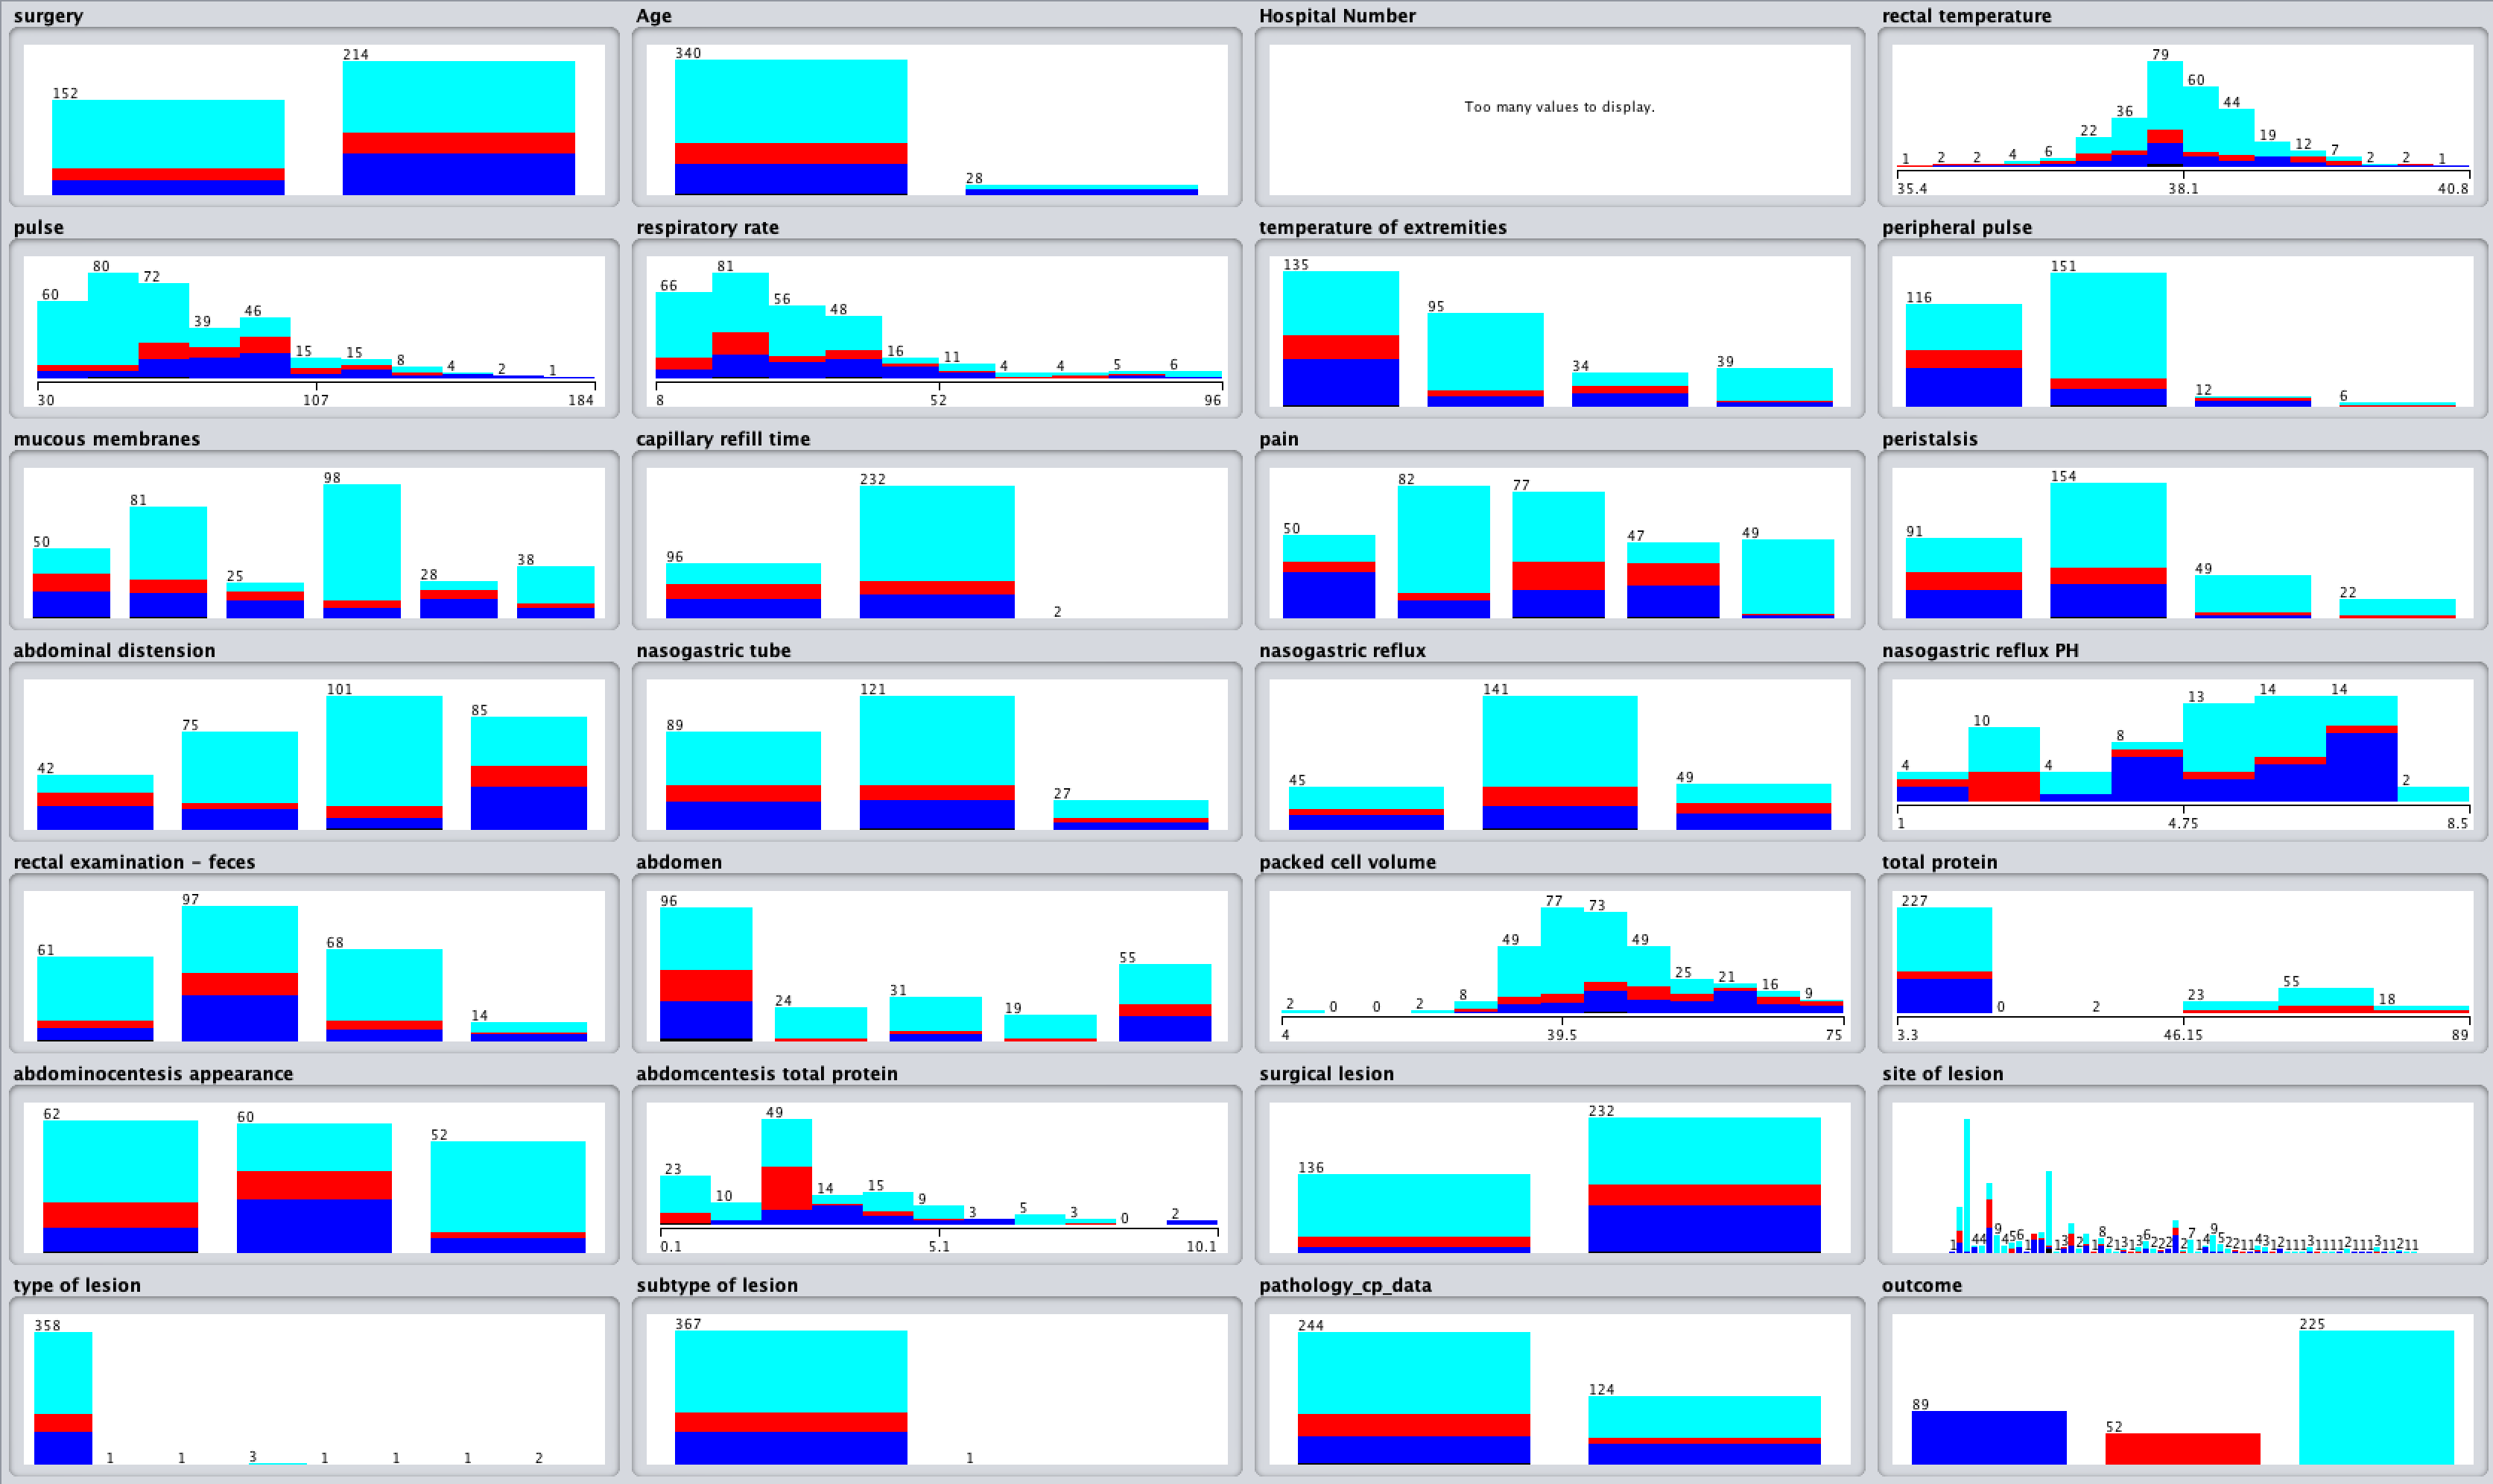
\includegraphics[width=17cm]{originalAttributeDistribution}
\caption{The original attribute value distribution}
\end{figure}
 

From the figure above, the attributes: \verb|Age|, \verb|Type of lesion| and \verb|Subtype of lesion| have a visibly uneven distribution. These attribute are removed before rule generation is started. The attribute \verb|pathology_cp_data| was described as being insignificant in the attribute information sheet and is therefore also removed.\\
Our objective is to find some interesting rules with relatively low support but high confidence that could help veterinarians with diagnosis and prognosis of digestive problems in horses.\\
The attribute \verb|outcome| is selected initially as the temporary class attribute. Even though association rule analysis does not rely on classes,  \verb|outcome| could be an interesting metric in the case of using association rule mining for classification.\\
The class value can always be changed in order to explore other interesting rules with different consequents.\\
In order to use the Apriori algorithm, all attributes have to be nominal. So the following attributes are discretized accordingly:
\begin{itemize}
\item The outcome values are renamed as:
\begin{itemize}
\item lived
\item died
\item was euthanized
\end{itemize}

\item The rectal temperature is discretized to throw out extreme values, using 8 bins.

\item The pulse attribute is also discretized. Here, 8 bins are used with equal frequency.

\item The respiratory rate is relabeled accordingly:
\begin{itemize}
\item Normal: 8-10 bpm
\item Above Normal: 11-25 bpm
\item Fast: 26-35 bpm
\item Extreme: Over 35 bpm
\end{itemize}

\item Total protein is discretized into 5 bins
\begin{itemize}
\item < 5.5 gms/dL
\item 5.5-6.4 gms/dL
\item 6.5-7.5 gms/dL
\item 7.6 - 10 gms/dL
\item > 10 gms/dL
\end{itemize}


\item Abdomcentesis total protein is split into 3 bins
\begin{itemize}
\item 0- 1.5 gms/dL
\item 1.6 - 3 gms/dL
\item > 3 gms/dL
\end{itemize}

\item packed cell volume is split into 3 bins
\begin{itemize}
\item $< 31 \%$
\item $31-50 \%$
\item $> 50 \%$
\end{itemize}

\item nasogastric reflux pH is split into 3 bins


\end{itemize}

Most of these attributes can be discretized with the \verb|MergeManyValues| filter (for numerical attribues).
